
% \pagebreak \ \pagebreak
\section{Our Approach} 

%Our work is similar to other approaches to mining
%repositories for developer networks, except that we explicitly focus on
%task-based communication as a more fine-grained method of connecting project
%members in the social networks. Box
%X places our work in the context of exiting approaches to
%building developer networks. 
% As a team manager, you are responsible for delivering
% a software product on time. 
% But Build 1 failed and your team needs to spend extra time diagnosing an integration issue and reworking code. 
% You suspect that your team failed to communicate important dependency which then broke the
% build. 
% To resolve this issue, social network analysis helps you to get insight into your teams communication.

To illustrate our approach of mining large repositories to construct social
networks that can help to solve team collaboration problems, we use the example
of a failed build. A social network is represented as a graph that consist of
nodes connected by edges. In our approach, the nodes represent people and edges
represent task-related communication between these people.

Figure \ref{fig:network} shows the step-by-step construction of our task-based
social networks. To explore the communication for Failed Build 1 (see left
column), we start with the project-wide people-artifact network. 
%R2.1
%The project-wide
%people-artifact network is composed of people and artifacts from available
%project repositories and their communication and contribution relationships. 
%
The project-wide people-artifact network is composed of artifacts, such as 
source code changes, emails, or documentation, that can be related to a task such as Bug 123.
Everyone that communicated about such an artifact or its respective task is included in the network
and connected to the task, that relates to the artifact.
%

We \emph{filter the people} from all teams who have contributed code to this
build. These people are Adam, Ines, Dillan, Gina, Eve, and Cathrin (coloured
blue). Then we \emph{filter the tasks} that were completed for this build, which
are GUI API, Bug 123, DataBase, Spell Check, and GUI Test. Using the task and
team member information, we complete the social network by connecting the people
for which we have recorded task-related communication. In this case we use
comments on tasks as communication records, represented as dashed lines between
team members and tasks in the figure.

By constructing and visualizing the task-based social network, represented as
blue lines in the bottom panel of the figure, it becomes apparent that there is a
missing communication connection between Cathrin and Eve. Cathrin was working on
the GUI API task, but never commented on the GUI Test task, and vice versa for
Eve. There may have been an important dependency between these two tasks that was
not communicated or resolved. You might conclude that this may have been part of
the problem that caused this build failure.

\subsection{Elements of Task-based Social Networks} 
Having informally described how social networks can be constructed from project
data, we now provide a high level description of how we conceptualize and
construct social networks for software teams. Our approach is repository and tool
independent and can be applied to any repositories that provide information about
people, tasks, technical artifacts, and communication. This include work, issue,
or change management repositories, such as Bugzilla or IBM Rational
ClearQuest\texttrademark; or source code management systems, such as CVS or IBM
Rational ClearCase\texttrademark; or even communication repositories such as
email archives.

We construct and analyze social networks within a \emph{collaboration scope} of
interest. In this example, around Failed Build 1, the collaboration scope is the
communication of the contributors to the failed build. Other examples include the
collaboration of people working on a critical task, in a particular geographical
location, or in a functional team such as testing.

There are three critical elements that are necessary to construct task-based
social networks for a collaboration scope and that need to be mined from software
development repositories:

\begin{description}
\item[Project Members] are people who work on the software project. These
\people s can be developers, testers, project managers, requirements analysts,
or clients. Project members, such as Cathrin and Eve, become nodes in the
social network.

\item[Collaborative Tasks] are units of work within the project that \people s
need to collaborate and communicate about. Examples of \cu s include resolving
Bug  123 or implementing the GUI API. More generally, implementing feature
requests and requirements can also be considered collaborative tasks.

\item[Task-related Communication] is the information exchanged while completing
a \cu\ and is the unique information that allows us to build task-based social
networks. In our example, dashed black lines represent task-related communication
such as a comment on Bug 123, or an email or chat message about GUI API.
Task-related communication is used to create the edges between \people s in the
social networks.
\end{description}

% \begin{figure}[!h]
% \begin{center}
% 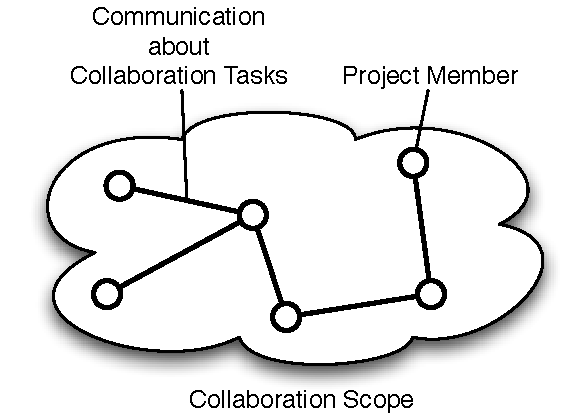
\includegraphics[width=8.0cm]{./figures/concepts}
% \label{fig:concept}
% \caption{Concept Visualization}
% \end{center}
% \end{figure}

\begin{figure*}[t!]
\begin{center}
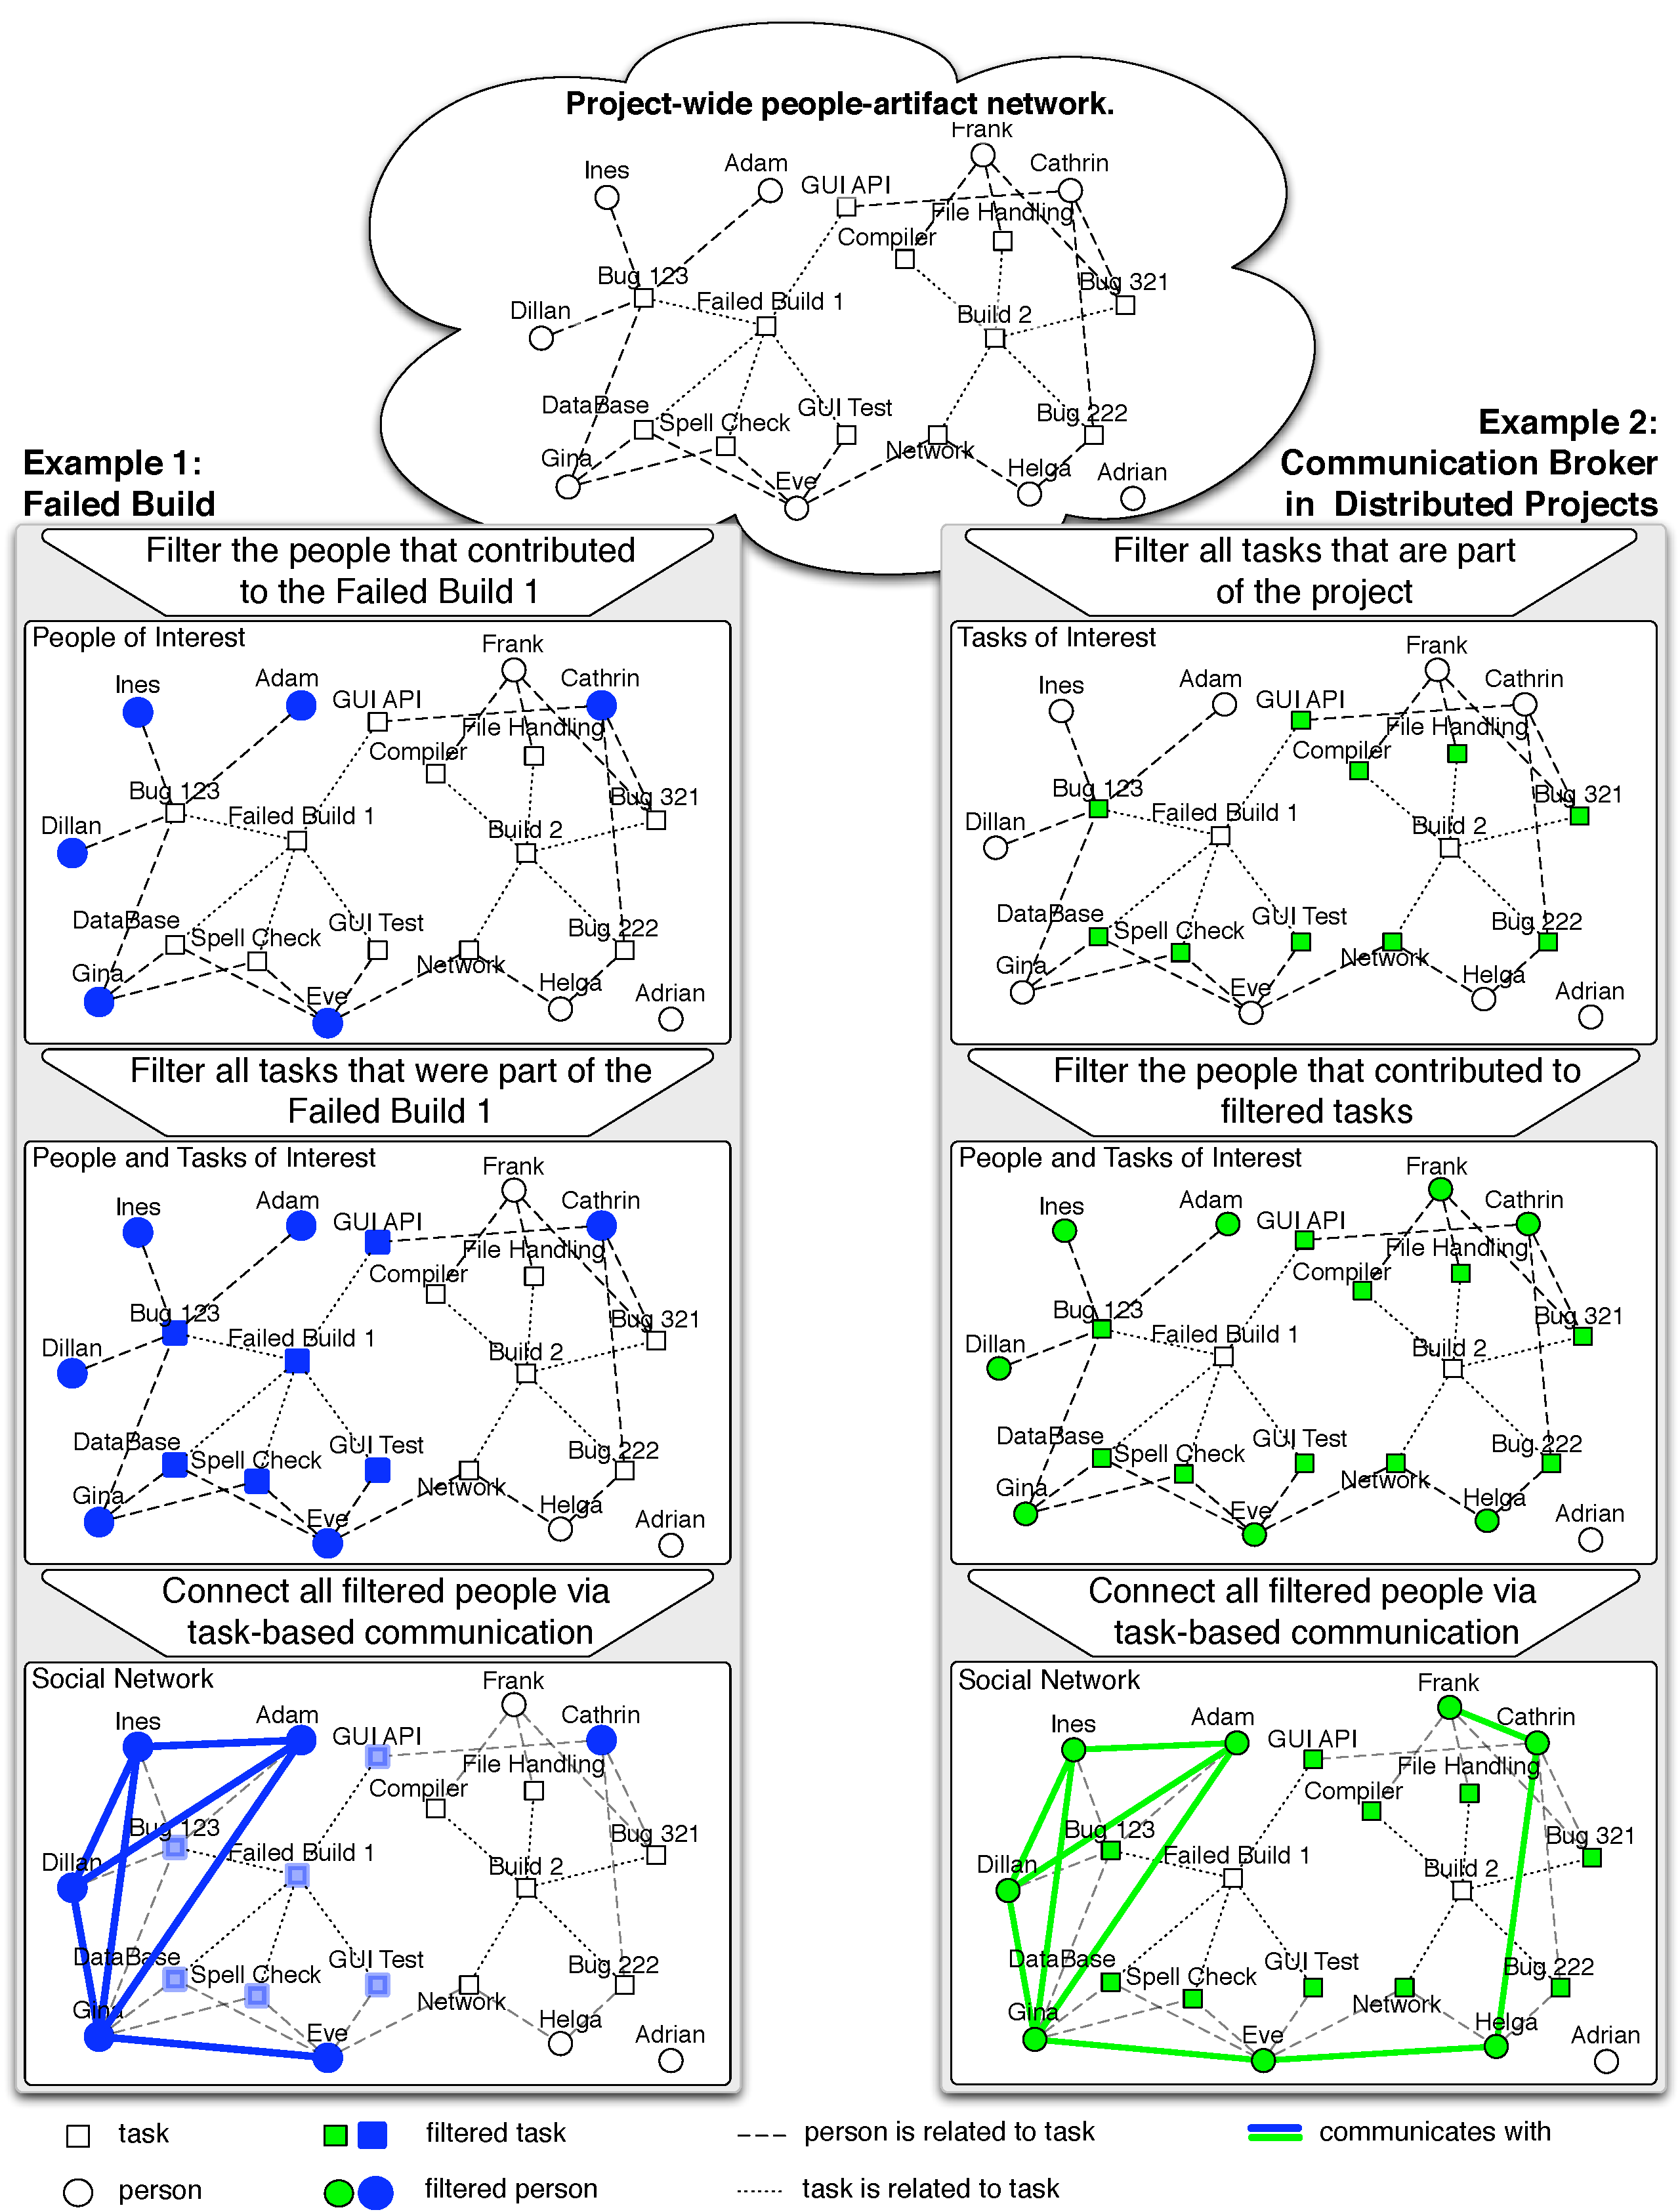
\includegraphics[height=0.9465\textheight]{./figures/grand_figure}
\caption{Social network construction examples in our approach}
\label{fig:network}
\end{center}
\end{figure*}

\subsection{Constructing Social Networks:}
The following three steps are used to construct a social network within a
collaboration scope: filtering of project members to identify nodes in the
network, filtering collaborative tasks to use as the context for collaboration,
and connecting project members to identify edges in the network. Each filtering
step includes criteria and reduces the set of \people s or \cu s from the entire
project. After collaborative tasks and team members are filtered, recorded
task-related communication is used to connect the nodes in the social network.

\paragraph{Filtering Project Members:}
To determine the set of nodes to be included in the social network we identify
those \people s that meet the criteria specified in the collaboration scope. In
our example, we restrict the team members to those who contributed to the failed
build, such as Adam, Eve, and Cathrin (coloured blue in Figure
\ref{fig:JazzProjectSN}). In addition, other constraints, such as temporal
% R2.1
constraints on when team members communicated about a task, can be added to
further reduce the included set of \people s.

\paragraph{Filtering Collaborative Tasks:}
Similar to the filtering of \people s, we use the criteria from the collaboration
scope to select \cu s. The \cu s provide the communication context used to
connect \people s in the following step. In our example, we restrict the tasks to
those included in Failed Build 1, such as GUI API, Bug 123, and GUI Test. The
filtering criteria can be based on properties of \cu s, such as task priority or
assigned team. Again, temporal constraints are often useful criteria, such as
selecting all development tasks contributed since the last build.

\paragraph{Connecting Project Members}
To connect \people s, creating edges in the social network, we leverage recorded
communication between the \people s in the filtered \cu s. For example, Gina and
Ines have both commented on Bug 123 and so we create an edge between them in the
social network. Our approach to constructing task-based social networks also
enables the inclusion of directed and weighted edges. Directed edges can
represent the direction of communication such as email sent from one team member
to another. Weighted edges can be used to represent the volume of communication
such as the number of emails sent.

\paragraph{}
While the filtering steps are independent, the order in which they are applied
can affect the composition of nodes and edges in the resulting social network.

\subsection{A Second Example -- Communication Brokers}
Here we provide a second example, applying project member and task filters in a
different order with differing criteria. This example demonstrates how social
networks can be used to find communication brokers between two project members.
This example is illustrated in the right column of Figure \ref{fig:network}.

Suppose, again, that you are the manager of a software team. Helga, a developer
in your project, complains that she needs information from Adam, but Adam has not
responded to information requests. Helga needs this information to complete her
work on Bug 222. You suspect that, due to time zone differences between
offices, Helga and Adam are rarely working at the same time and have trouble
communicating effectively. Social network analysis can identify other people in
the project that may be able to broker communication between Helga and Adam.

To construct a social network for this application, we filter the collaborative
tasks in the project keeping all tasks (coloured green in the right column of
Figure \ref{fig:network}). Then we filter the project members, keeping those that
have contributed to those collaborative tasks. Finally, using the recorded
task-based communication, we connect the project members to create a social
network for the entire project. By visualizing this social network we see that
Gina and/or Eve are good candidates to broker communication between Helga and
Adam. Choosing to use either Gina or Eve as a communication broker could be done
based on their geographic location with respect to Adam.

\paragraph{}
These two examples illustrate how the same repository could be mined for two
different collaboration scopes of interest to construct two different social
networks. An overview of software repository mining approaches to generate
developer networks are outlined in the Constructing Developer Networks sidebar.
